\subsection{P-Regler} % (fold)
\label{sub:P-Regler}
\begin{frame}
    \frametitle{P-Regler}
    \framesubtitle{}
    \begin{block}{Versuchsziel}
         \begin{itemize}
             \item Untersuchen verschiedener $k_p$ Werte für P-Regler
         \end{itemize}
    \end{block}
\end{frame}
\begin{frame}
    \frametitle{P-Regler}
    \framesubtitle{$k_p=5$}
    \begin{columns}[c]
        \column{0.4\textwidth}
            \begin{block}{Verhalten}
                 \begin{itemize}
                     \item Schrittgröße zu hoch
                     \item konstantes "Über-/Unterspringen" des Limits
                 \end{itemize}
            \end{block}
        \column{0.6\textwidth}
        \begin{figure}[H]
        \begin{center}
                \includegraphics[scale=0.4]{./img/plots/Auf_2_b_5.eps}
        \end{center}
        \end{figure}
     \end{columns}
\end{frame}
\begin{frame}
    \frametitle{P-Regler}
    \framesubtitle{$k_p=5$}
    \begin{columns}[c]
        \column{0.4\textwidth}
            \begin{block}{Verhalten}
                \begin{itemize}
                    \item Schrittgröße zu klein
                    \item Korrektur kann nicht für Wärmeabgabe kompensieren
                    \item Stagnation weit unter Ziel
                \end{itemize}
            \end{block}
        \column{0.6\textwidth}
        \begin{figure}[H]
        \begin{center}
                \includegraphics[scale=0.4]{./img/plots/Auf_2_b_0_1.eps}
        \end{center}
        \end{figure}
     \end{columns}
\end{frame}
\begin{frame}
    \frametitle{P-Regler}
    \framesubtitle{$k_p=5$}
    \begin{columns}[c]
        \column{0.4\textwidth}
            \begin{block}{Verhalten}
                \begin{itemize}
                    \item Schrittgröße liegt im Mittelbereich
                    \item trotzdem Stagnation weit unterhalb Ziel
                \end{itemize}
            \end{block}
        \column{0.6\textwidth}
        \begin{figure}[H]
        \begin{center}
                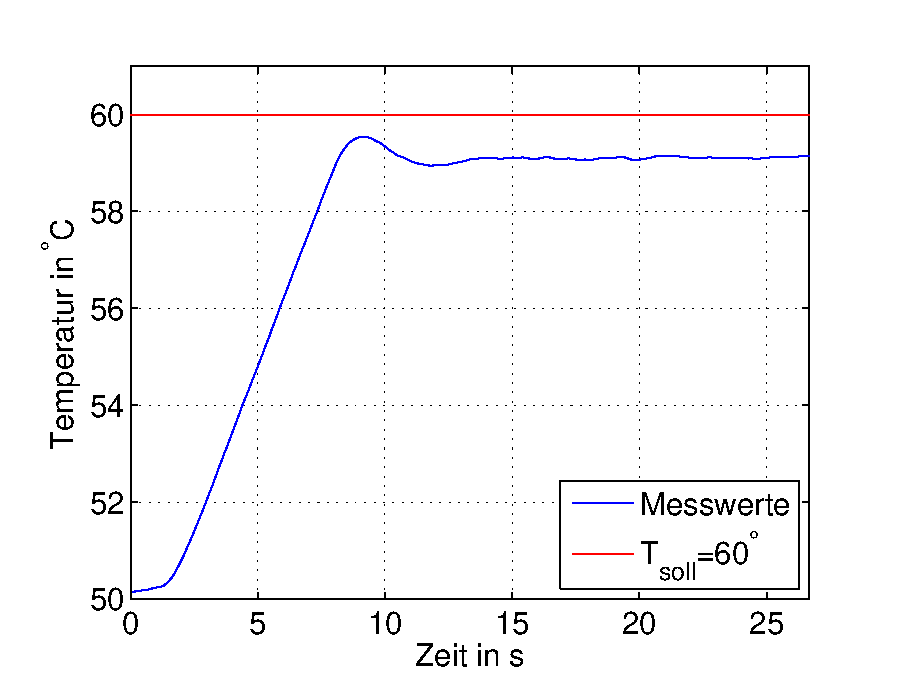
\includegraphics[scale=0.4]{./img/plots/Auf_2_b_1.eps}
        \end{center}
        \end{figure}
     \end{columns}
\end{frame}
\begin{frame}
    \frametitle{Wieso stagniert $k_p = 1$? unter dem Ziel}
    \framesubtitle{}
    \begin{columns}[c]
        \column{0.6\textwidth}
            \begin{block}{Verhalten}
                \begin{itemize}
                    \item P ist stets positiv
                    \item P sinkt linear bis nah an $T=60^{\circ}C$
                    \item $P=K_p(W-X)$ wird zu klein um für Abkühlung zu
                    kompensieren (vgl. $k_p=0.1$)
                    \item P schwingt zurück auf $T_0 < 60^{\circ}C$ und
                    stagniert
                \end{itemize}
            \end{block}
            \begin{alertblock}{}
                P-Regulierung alleine kann niemals das Limit erreichen
            \end{alertblock}
        \column{0.6\textwidth}
            \begin{figure}[H]
            \begin{center}
                    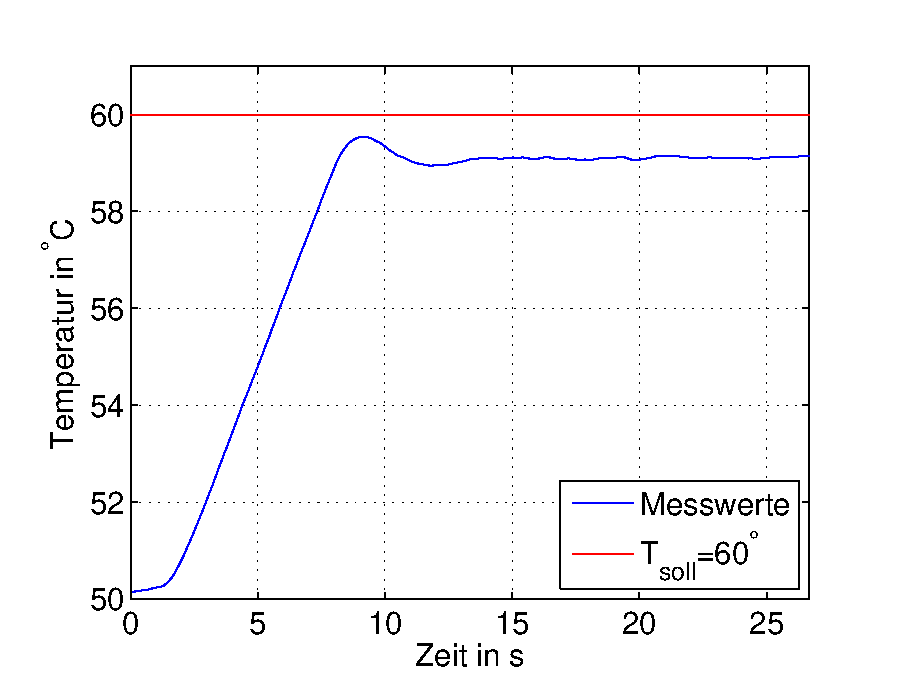
\includegraphics[scale=0.3]{./img/plots/Auf_2_b_1.eps}
            \end{center}
            \end{figure}
            \begin{figure}[H]
            \begin{center}
                    \includegraphics[scale=0.3]{./img/plots/Auf_2_b_1_P.eps}
            \end{center}
            \end{figure}
     \end{columns}
\end{frame}
% subsection P-Regler (end)
